\documentclass[conference,a4paper]{IEEEtran}
\usepackage[utf8]{inputenc}
\usepackage[T1]{fontenc}
\usepackage[english]{babel}
\usepackage{amsmath,amssymb}
\usepackage{graphicx}
\usepackage{booktabs}
\usepackage{array}
\usepackage{siunitx}
\usepackage{listings}
\usepackage{xcolor}
\usepackage[hidelinks]{hyperref}
\lstset{basicstyle=\ttfamily\scriptsize, breaklines=true, frame=single, columns=fullflexible,
        keywordstyle=\color{blue!60!black}, commentstyle=\color{green!40!black}, language=C++}
\graphicspath{{figuras/}}

\raggedbottom
\begin{document}

\title{Luenberger and Kalman Observers and Discrete Position Control of the Elbow Joint of a SCARA Robot}

\author{\IEEEauthorblockN{Andrés Ramírez\qquad Simón Patiño\qquad Jeronimo Valencia\\ Jorge Alejandro de Santiago}
\IEEEauthorblockA{Mechatronics Engineering -- Digital Control\\
Universidad EIA, Envigado, Colombia}}

\maketitle

\begin{abstract}
Two discrete state observers, a full-order predictor Luenberger observer and a linear Kalman filter, are designed and implemented to estimate the armature current and the speed of a Pololu 37D \#4753 (50:1) gearmotor, measuring only the speed with an incremental encoder. The parametric model from the previous laboratory is tuned so that it draws \SI{0.2}{A} and reaches the nominal speed at \SI{12}{V}, and it is refined with steps measured on the elbow joint of a SCARA robot. With the same model, a discrete PID position controller is designed directly in the $z$-plane by pole placement, with a reference prefilter and anti-windup. Everything runs on a Raspberry Pi Pico with a \SI{10}{ms} sampling period and is operated from a web interface that allows changing the reference live. Both observers give consistent current estimates; under disturbances the Kalman filter tracks the speed with a \SI{7.8}{rad/s} RMS error, against \SI{34.8}{rad/s} for the Luenberger observer, and its covariance converges in three samples. Over 27 measured steps, the position loop settles in \SIrange{0.74}{0.85}{s} with less than \SI{1}{\percent} overshoot, against \SIrange{0.65}{0.75}{s} in the design.
\end{abstract}

\begin{IEEEkeywords}
Luenberger observer, Kalman filter, discrete control, pole placement, PID, DC motor, Raspberry Pi Pico.
\end{IEEEkeywords}

\section{Introduction}
In many applications not every variable of a system can be measured, either because no sensor is available or because measuring it is expensive. In a DC motor the speed is easily obtained with an encoder, but the armature current requires an additional sensor. A state observer reconstructs the unmeasured states from the system model, the input and the measured outputs \cite{ogata}.

This work implements the two observers proposed in the laboratory guide \cite{guia,guiaeia}: the Luenberger observer, designed by pole placement with Ackermann's formula, and the linear Kalman filter, designed from the model and measurement uncertainty \cite{welch}. Unlike the guide, which uses a myRIO board and LabVIEW, the implementation runs on a Raspberry Pi Pico driving the elbow motor of a SCARA robot. Table~\ref{tab:actividades} lists the four activities of the guide's procedure and where each one is reported. As additional work beyond the guide, a discrete-time position controller is designed with the same discrete model, so that the observers are also evaluated with the motor in closed loop (Sections~VI and~VIII-D).

\begin{table}[!t]
\centering
\caption{Activities of the Laboratory Procedure}
\label{tab:actividades}
\begin{tabular}{>{\raggedright\arraybackslash}p{0.56\columnwidth}>{\raggedright\arraybackslash}p{0.32\columnwidth}}
\toprule
Activity of the guide \cite{guia} & Where \\
\midrule
1. Tune the parametric model to the measured data & Sec.~IV-B, Fig.~\ref{fig:ajuste}, Table~\ref{tab:param} \\
2. State space, simulation of current and speed, \SI{0.2}{A} and nominal speed at \SI{12}{V}, comparison with the measurements & Sec.~IV-B, Figs.~\ref{fig:nominal} and~\ref{fig:ajuste} \\
3. Luenberger observer from the speed measurement & Sec.~V-A, VIII-A/B, Figs.~\ref{fig:polos}--\ref{fig:pert} \\
4. Linear Kalman filter from the speed measurement & Sec.~V-B, VIII-A--C, Figs.~\ref{fig:sim}--\ref{fig:traza} \\
Additional: discrete position control & Sec.~VI, VIII-D, Figs.~\ref{fig:pid}, \ref{fig:posreal} \\
\bottomrule
\end{tabular}
\end{table}

\section{Theoretical Framework}
\subsection{DC Motor Model}
With the states $x=[i_a\;\;\omega]^T$, the input $u=V_a$ and the measured output $y=\omega$, the motor equations are
\begin{align}
\dot{i}_a &= -\frac{R_a}{L_a} i_a - \frac{K_v}{L_a}\omega + \frac{1}{L_a}V_a,\\
\dot{\omega} &= \frac{K_v}{J} i_a - \frac{\beta}{J}\omega,
\end{align}
that is, $\dot{x}=A_c x + B_c u$, $y = Cx$ with
\begin{equation}
A_c=\begin{bmatrix}-\frac{R_a}{L_a} & -\frac{K_v}{L_a}\\[2pt] \frac{K_v}{J} & -\frac{\beta}{J}\end{bmatrix},\quad
B_c=\begin{bmatrix}\frac{1}{L_a}\\[2pt] 0\end{bmatrix},\quad
C=\begin{bmatrix}0 & 1\end{bmatrix}.
\end{equation}

\subsection{Discretization}
Since the Pico holds the voltage constant between samples, the actuator is a zero-order hold with sampling period $T_s$:
\begin{equation}
A = e^{A_c T_s},\qquad B=\int_0^{T_s} e^{A_c\tau}\,d\tau\, B_c,
\end{equation}
\begin{equation}
x_k = A x_{k-1} + B u_{k-1},\qquad y_k = C x_k .
\end{equation}
Each continuous pole $s$ maps to $z=e^{sT_s}$; a mode much faster than $T_s$ ends up at $z\approx0$.

\subsection{Luenberger Observer}
The full-order predictor observer uses the input and the measurement from the previous sample:
\begin{equation}
\hat{x}_k = (A-LC)\hat{x}_{k-1} + L\,y_{k-1} + B\,u_{k-1}.
\label{eq:luen}
\end{equation}
The estimation error evolves as $e_k=(A-LC)e_{k-1}$, so $L$ is chosen to place the eigenvalues of $A-LC$ inside the unit circle. With Ackermann's formula,
\begin{equation}
L = \Phi(A)\,\mathcal{O}^{-1}\begin{bmatrix}0\\1\end{bmatrix},\qquad \mathcal{O}=\begin{bmatrix}C\\CA\end{bmatrix},
\end{equation}
where $\Phi(z)$ is the desired characteristic polynomial.

\subsection{Linear Kalman Filter}
Starting from $\hat{x}_0$ and $P_0$, each sample performs a prediction and a correction \cite{welch}:
\begin{align}
\hat{x}_k^- &= A\hat{x}_{k-1}^+ + B u_{k-1}, & P_k^- &= A P_{k-1}^+ A^T + Q,\\
K_k &= P_k^- C^T (C P_k^- C^T + R)^{-1}, & &\\
\hat{x}_k^+ &= \hat{x}_k^- + K_k(y_k - C\hat{x}_k^-), & P_k^+ &= (I-K_kC)P_k^- ,
\end{align}
where $Q$ represents the model uncertainty and $R$ the measurement variance. $P_k$ is the covariance of the estimation error. To follow its evolution with a single number,
\begin{equation}
p_k=\sqrt{P_{11,k}^2+P_{22,k}^2},
\label{eq:traza}
\end{equation}
the norm of its diagonal, is used. If $p_k$ grows without bound the filter diverges; if it decreases and settles, the filter converges. With constant $A$, $Q$ and $R$, $P_k$ follows the Riccati equation and converges to a fixed value that does not depend on the measurements \cite{welch}; this is why it does not go to zero.

\subsection{Discrete Control by Pole Placement}
Let the position plant be $G(z)=N(z)/D(z)$ and the controller
\begin{equation}
C(z)=\frac{U(z)}{E(z)}=\frac{q_0z^2+q_1z+q_2}{(z-1)(z+g)},
\label{eq:pid}
\end{equation}
which is a discrete PID with a filtered derivative: the pole at $z=1$ gives the integral action and the pole at $z=-g$ filters the derivative. The closed loop has the characteristic polynomial
\begin{equation}
(z-1)(z+g)D(z)+N(z)\,(q_0z^2+q_1z+q_2)=\Phi_c(z),
\label{eq:diof}
\end{equation}
which is linear in $g,q_0,q_1,q_2$. If $D(z)$ is second order, matching coefficients with the fourth-order desired polynomial $\Phi_c(z)$ gives four equations in four unknowns \cite{astrom}. The desired poles come from continuous-time specifications: the dominant pair $s=-\sigma\pm j\omega_d$, with $\sigma=4/t_s$ and $\omega_d=\sigma\sqrt{1-\zeta^2}/\zeta$, maps to the $z$-plane as $z=e^{sT_s}$. Solving \eqref{eq:pid} for $u$ gives the difference equation
\begin{equation}
u_k=(1-g)u_{k-1}+g\,u_{k-2}+q_0e_k+q_1e_{k-1}+q_2e_{k-2}.
\label{eq:dif}
\end{equation}
If the already saturated voltage is stored in $u_{k-1}$ and $u_{k-2}$, the integral part does not accumulate while the actuator is at its limit (anti-windup).

\section{Experimental Setup}
The elbow motor of a SCARA RRP robot is used: a \SI{12}{V} Pololu 37D \#4753 gearmotor with a 50:1 gearbox \cite{pololu}, which drives the forearm through a 3:1 pulley. The Hall encoder gives 64 counts per revolution of the motor shaft. The speed is computed as the position difference between two samples divided by $T_s$, so its resolution is $2\pi/(64\,T_s)\approx\SI{9.8}{rad/s}$. At the elbow, the angular resolution is $2\pi/(64\cdot150)\approx\SI{0.65}{mrad}$. The motor is driven by a BTS7960 H-bridge with a \SI{20}{kHz} PWM from a Raspberry Pi Pico, which reads the encoder with a PIO state machine.

The firmware runs a loop every $T_s=\SI{10}{ms}$ that measures, updates both observers, computes the voltage (fixed in the open-loop experiments, or given by the position controller) and sends the data over USB. Since the elbow has a limited travel (about \SI{3.7}{rad}), the firmware homes against the limit switch, cuts the voltage before either end of travel and stops the motor if it stalls. The prismatic axis is kept braked. When the elbow accelerated, its reaction torque turned the shoulder; therefore the shoulder is held by its own PD loop ($u=30\,e-1.0\,\omega$, \SI{4}{V} limit), which runs in a \SI{10}{ms} interrupt independent of the elbow loop and releases if the shoulder moves more than \SI{0.15}{rad} away.

On the PC, a Python server keeps the serial port open and a web page sends the commands (\emph{home}, voltage steps or \texttt{pos REF T}) and plots the angle, the speed, the estimated currents, the voltage and $p_k$ live. During a position run, the reference can be changed without stopping the loop (\texttt{r REF}). Each run is saved to a CSV file.

\section{Motor Model}
\subsection{Laboratory 1 Model}
The previous parametric identification gave the parameters in the Lab~1 column of Table~\ref{tab:param}, with an armature resistance of \SI{72.7}{\ohm}. With that model the motor reaches \SI{0.084}{A} and \SI{558}{rad/s} (\SI{107}{rpm} at the output) at \SI{12}{V}, far from the \SI{0.2}{A} and \SI{200}{rpm} specified by the manufacturer. $K_v$ and $\beta$ were consistent with the datasheet, but $R_a$ was about 30 times larger than the value derived from the stall current (\SI{5.5}{A} at \SI{12}{V}).

\subsection{Model Tuning}
$R_a$ was set to $12/5.5 = \SI{2.18}{\ohm}$, and the two steady-state conditions of the guide were imposed, $i_a=\SI{0.2}{A}$ and $\omega=\omega_{nom}=\SI{1047}{rad/s}$ (\SI{10000}{rpm} at the motor shaft), which gives
\begin{equation}
K_v=\frac{12-R_a\,i_a}{\omega_{nom}},\qquad \beta = \frac{K_v\, i_a}{\omega_{nom}}.
\end{equation}
$J$ and $L_a$ were then fitted by least squares to reproduce three steps of 4, 6 and \SI{8}{V} measured on the elbow. The resulting $J$ includes the forearm inertia reflected to the motor shaft. Table~\ref{tab:param} summarizes the parameters.

\begin{table}[!t]
\centering
\caption{Motor Parameters}
\label{tab:param}
\begin{tabular}{lcc}
\toprule
Parameter & Lab 1 & Tuned \\
\midrule
$R_a$ (\si{\ohm}) & 72.7 & 2.18 \\
$L_a$ (\si{H}) & \num{6.62e-2} & \num{5.56e-4} \\
$K_v$ (\si{V.s/rad}) & \num{1.06e-2} & \num{1.104e-2} \\
$J$ (\si{kg.m^2}) & \num{8.55e-7} & \num{2.81e-6} \\
$\beta$ (\si{N.m.s}) & \num{1.59e-6} & \num{2.11e-6} \\
\midrule
$i_a$ at \SI{12}{V} (\si{A}) & 0.084 & 0.200 \\
$\omega$ at \SI{12}{V} (\si{rad/s}) & 558 & 1047 \\
$\tau_{mech}$ (\si{ms}) & 273 & 48 \\
\bottomrule
\end{tabular}
\end{table}

With these values,
\begin{equation}
A_c=\begin{bmatrix}-3924.1 & -19.86\\ 3935.3 & -0.752\end{bmatrix},\quad B_c=\begin{bmatrix}1798.6\\0\end{bmatrix},
\end{equation}
and with $T_s=\SI{10}{ms}$,
\begin{equation}
A=\begin{bmatrix}-0.00419 & -0.00415\\ 0.8233 & 0.8166\end{bmatrix},\quad B=\begin{bmatrix}0.3793\\ 15.991\end{bmatrix}.
\end{equation}
The discrete plant poles are $z\approx0$ (electrical mode, $\tau_e=L_a/R_a\approx\SI{0.25}{ms}\ll T_s$) and $z=0.812$ (mechanical mode). Fig.~\ref{fig:nominal} verifies the nominal condition and Fig.~\ref{fig:ajuste} compares the model with the data.

\begin{figure}[!t]
\centering
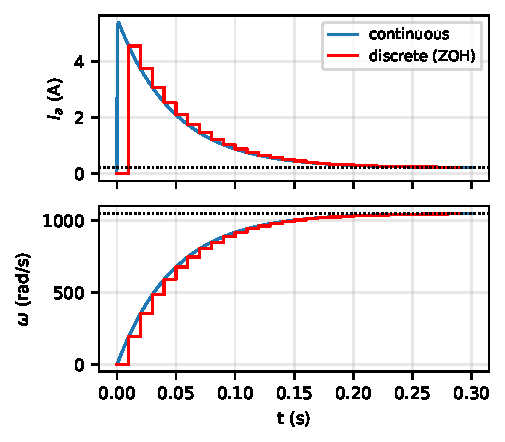
\includegraphics[width=\columnwidth]{nominal.pdf}
\caption{Response of the tuned model to \SI{12}{V}: the current settles at \SI{0.2}{A} and the speed at \SI{1047}{rad/s}.}
\label{fig:nominal}
\end{figure}

\begin{figure}[!t]
\centering
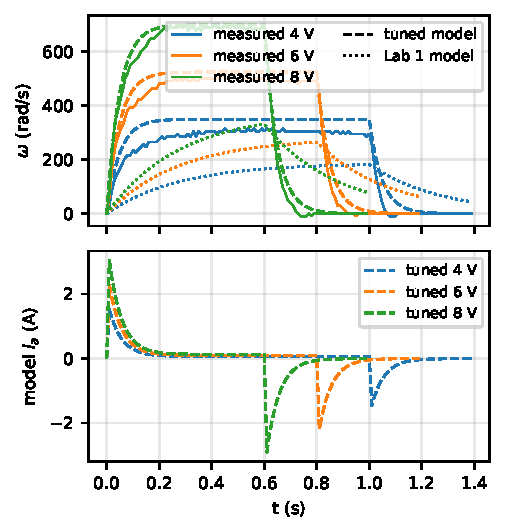
\includegraphics[width=\columnwidth]{ajuste.pdf}
\caption{Steps of 4, 6 and \SI{8}{V} measured on the elbow, compared with the Lab 1 model (dotted) and with the tuned model (dashed).}
\label{fig:ajuste}
\end{figure}

The tuned model reproduces the measured time constant, but overestimates the speed by about \SI{40}{rad/s} at \SI{4}{V}. The measured steady-state speeds (305, 496 and \SI{687}{rad/s}) grow by about \SI{96}{rad/s} per volt, and extrapolated to \SI{12}{V} they give $\approx\SI{1070}{rad/s}$, close to the nominal speed. However, the line does not pass through the origin: there is a dead zone of about \SI{0.8}{V} caused by the dry friction of the gearbox and the arm, which a linear model cannot represent.

\section{Observer Design}
\subsection{Luenberger}
The observability matrix
\begin{equation}
\mathcal{O}=\begin{bmatrix}C\\ CA\end{bmatrix}=\begin{bmatrix}0 & 1\\ 0.8233 & 0.8166\end{bmatrix},\qquad \det\mathcal{O}=-0.8233,
\end{equation}
has rank 2, so the system is observable from the speed measurement alone. The initial design, with poles at $z=0.3$ and $0.4$, produced negative current estimates down to \SI{-3.5}{A} with the real data (Fig.~\ref{fig:polos}). The reason is that the electrical pole of the plant is already at $z\approx0$: moving it to $0.3$ makes the current mode of the observer slower than that of the plant, and the small model error (the friction) accumulates in the current. The poles $z=\{0,\;0.2\}$ were therefore chosen, which keep the electrical pole and speed up the mechanical one, giving
\begin{equation}
\Phi(z)=z^2-0.2z,\qquad L=\begin{bmatrix}-0.00312\\ 0.6124\end{bmatrix}.
\end{equation}

\begin{figure}[!t]
\centering
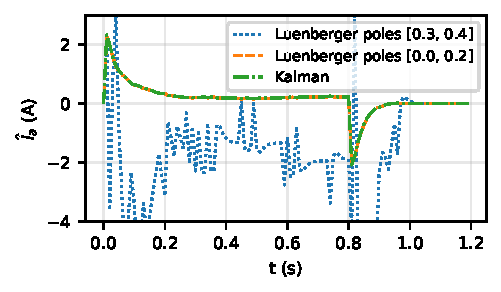
\includegraphics[width=\columnwidth]{polos.pdf}
\caption{Estimated current with the data of the \SI{6}{V} step: with the poles $\{0.3,0.4\}$ the Luenberger observer gives negative currents; with $\{0,0.2\}$ it matches the Kalman filter.}
\label{fig:polos}
\end{figure}

\subsection{Kalman}
The measurement variance was taken from the steady-state data of the steps, between 26 and \SI{45}{(rad/s)^2}, and $R=35$ was used. For the model, an uncertainty of \SI{10}{mA} in the current and \SI{10}{rad/s} in the speed was assumed, and the initial estimate was given a larger uncertainty in the current, which is not measured:
\begin{equation}
Q=\begin{bmatrix}10^{-4} & 0\\ 0 & 100\end{bmatrix},\quad P_0=\begin{bmatrix}0.1 & 0\\ 0 & 100\end{bmatrix}.
\end{equation}
The gain converges to $K=[-5.98\times10^{-4}\;\;0.771]^T$. No retuning was needed with these values.

\section{Position Controller Design (Additional Work)}
\subsection{Discrete Plant}
The elbow angle, $\dot{\theta}=\omega/150$ (50:1 gearbox and 3:1 pulley), is added to the model of Section~IV, and the result is discretized with a zero-order hold. The transfer function from voltage to angle is third order, but the electrical pole ($z\approx10^{-17}$) cancels with a zero at $z=-0.0012$, which leaves
\begin{equation}
G(z)=\frac{\theta(z)}{U(z)}=\frac{5.372\times10^{-4}\,(z+1.029)}{(z-1)(z-0.8124)}.
\label{eq:planta}
\end{equation}
The pole at $z=1$ is the integrator (the position is the integral of the speed) and the one at $z=0.8124$ is the mechanical mode. The zero at $z=-1.029$ is a sampling zero introduced by the hold; since it lies outside the unit circle, the design does not cancel it.

\subsection{Controller}
The specifications $\zeta=0.7$ (about \SI{5}{\percent} overshoot) and $t_s=\SI{0.5}{s}$ give $\sigma=\SI{8}{s^{-1}}$, $\omega_d=\SI{8.16}{rad/s}$ and the dominant pair $z=0.9231\,e^{\pm j0.0816}=0.920\pm0.075j$. The two remaining poles were placed at $z=0.6$, faster than the dominant pair. Solving \eqref{eq:diof} with \eqref{eq:planta} gives
\begin{align}
q_0&=139.71, & q_1&=-247.97,\\
q_2&=110.03, & g&=-0.3027,
\end{align}
and it was verified that the closed-loop poles lie exactly at the requested values.

\subsection{Reference Prefilter}
Since $q_0$ is large, a \SI{1}{rad} reference step would ask for more than \SI{100}{V}. With the saturation at $\pm\SI{6}{V}$, in simulation the voltage jumped from $+6$ to \SI{-6}{V} between two samples, with current peaks of $\pm\SI{3}{A}$, because the saturated loop is no longer linear. The reference therefore goes first through a second-order prefilter outside the loop,
\begin{equation}
F(z)=\left(\frac{(1-\alpha)z}{z-\alpha}\right)^2,\qquad \alpha=0.93,
\end{equation}
with time constant $-T_s/\ln\alpha\approx\SI{0.14}{s}$. The prefilter does not change the closed-loop poles: it only smooths the reference that enters the loop. In simulation, with $V_{max}=\SI{6}{V}$, steps from 0.5 to \SI{2.2}{rad} settle in \SIrange{0.65}{0.75}{s} without overshoot.

\section{Implementation}
The observer matrices and the controller coefficients are computed in Python and written to header files that the firmware compiles. Since $C=[0\;1]$, the innovation is a scalar and the Kalman filter needs no matrix inversion. The Luenberger observer step is:
\begin{lstlisting}
// x(k) = (A - L C) x(k-1) + L y(k-1) + B u(k-1)
float e  = y_ant - x[1];
float x0 = AD[0]*x[0] + AD[1]*x[1] + BD[0]*u_ant + LG[0]*e;
float x1 = AD[2]*x[0] + AD[3]*x[1] + BD[1]*u_ant + LG[1]*e;
\end{lstlisting}
the Kalman filter correction:
\begin{lstlisting}
float s  = Pm[3] + RK;            // C P- C' + R
float K0 = Pm[1]/s, K1 = Pm[3]/s; // gain
float e  = y - x1;                // innovation
x[0] = x0 + K0*e;  x[1] = x1 + K1*e;
\end{lstlisting}
and the position controller, with the prefilter and the difference equation \eqref{eq:dif}:
\begin{lstlisting}
rf1 = a*rf1 + (1-a)*ref;          // prefilter F(z)
rf  = a*rf  + (1-a)*rf1;
float e = rf - art;               // error in rad
float u = (1-g)*u1 + g*u2 + q0*e + q1*e1 + q2*e2;
u = limitar(u, -vmax, vmax);      // u1, u2 keep the saturated u
e2 = e1; e1 = e;
\end{lstlisting}
The \SI{10}{ms} loop includes the measurement, both observers, the controller, the protections and the data transmission, including $p_k$ from \eqref{eq:traza}.

\section{Results}
\subsection{Observers: Simulation with Measured Data}
Before the implementation, both observers were run on the measured steps with the same algorithm as the firmware (Fig.~\ref{fig:sim}). Over the three steps the speed RMS error was 12--14~rad/s for Luenberger and 2.6--3.1~rad/s for Kalman. The estimated steady-state currents agreed between both methods (0.27, 0.23 and \SI{0.19}{A} at 4, 6 and \SI{8}{V}).

\begin{figure}[!t]
\centering
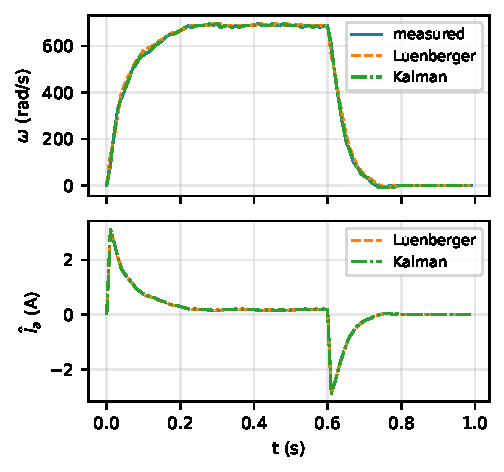
\includegraphics[width=\columnwidth]{simulacion.pdf}
\caption{Simulation of the observers on the measured \SI{8}{V} step.}
\label{fig:sim}
\end{figure}

\subsection{Observers on the Pico in Open Loop}
Fig.~\ref{fig:escalon} shows a \SI{5}{V} step estimated in real time. Both observers follow the measured speed, and the estimated current shows the start-up peak (\SI{1.9}{A}), settles at \SI{\approx0.25}{A} and becomes negative during braking.

\begin{figure}[!t]
\centering
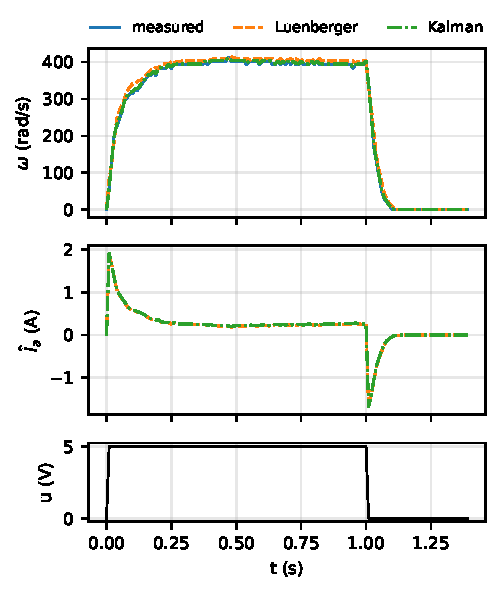
\includegraphics[width=\columnwidth]{real_escalon.pdf}
\caption{Implementation on the Pico: \SI{5}{V} step for \SI{1}{s}.}
\label{fig:escalon}
\end{figure}

Under voltage changes of 4, 8, 3, $-6$ and \SI{-3}{V} (Fig.~\ref{fig:perfil}), the observers follow the speed in every segment, including the direction reversal. The estimated current shows a peak at each change and reaches \SI{-3}{A} when the direction reverses, which is the expected behavior of a DC motor.

\begin{figure}[!t]
\centering
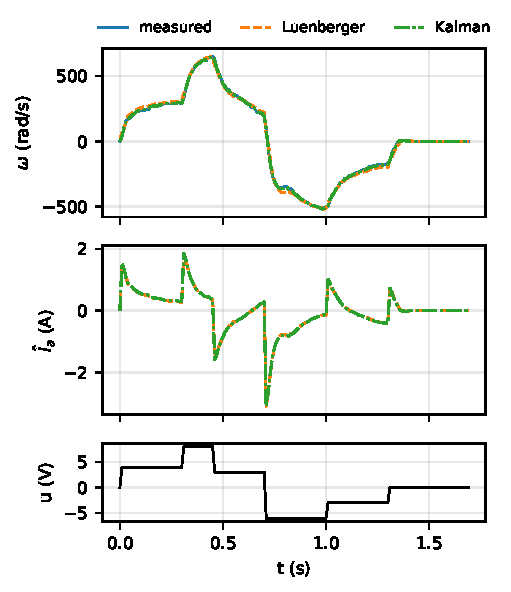
\includegraphics[width=\columnwidth]{real_perfil.pdf}
\caption{Voltage changes: 4, 8, 3, $-6$, $-3$ and \SI{0}{V}.}
\label{fig:perfil}
\end{figure}

For the disturbance test, the elbow moves back and forth at $\pm\SI{3.5}{V}$ for \SI{6}{s}, reversing at 0.5 and \SI{1.4}{rad}, while the forearm is braked by hand (Fig.~\ref{fig:pert}). Each time the load is applied, the measured speed drops and the estimated current rises from \SI{\approx0.4}{A} to 1.0--\SI{1.3}{A}. That value approaches the stall current at \SI{3.5}{V} ($3.5/R_a\approx\SI{1.6}{A}$). Table~\ref{tab:rms} summarizes the errors.

\begin{figure}[!t]
\centering
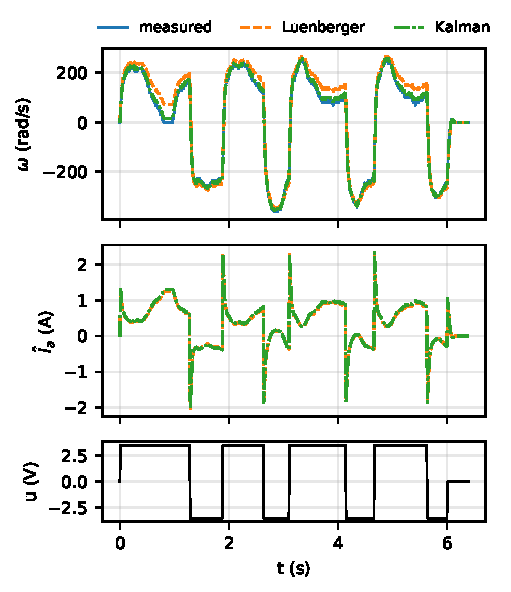
\includegraphics[width=\columnwidth]{real_perturbacion.pdf}
\caption{Disturbance: the elbow moves back and forth at $\pm\SI{3.5}{V}$ and is braked by hand three times.}
\label{fig:pert}
\end{figure}

\begin{table}[!t]
\centering
\caption{RMS Error of the Estimated Speed (\si{rad/s})}
\label{tab:rms}
\begin{tabular}{lcc}
\toprule
Test & Luenberger & Kalman \\
\midrule
4, 6 and \SI{8}{V} steps (simulation) & 12--14 & 2.6--3.1 \\
Load disturbance (Pico) & 34.8 & 7.8 \\
\bottomrule
\end{tabular}
\end{table}

\subsection{Convergence of the Kalman Covariance}
Fig.~\ref{fig:traza} shows $p_k$ computed on the Pico. It starts at $p_{-1}=100$ (the initial estimate $P_0$), drops to 28.93 at the first correction and to 27.06 at the second, and from the third sample on it stays at $p=26.99$, which corresponds to $P_{11}=\SI{5.1e-4}{A^2}$ and $P_{22}=\SI{26.99}{(rad/s)^2}$. The value does not change with the reference steps or with the load, as expected from a linear filter with constant $Q$ and $R$: the filter quickly converges to a steady uncertainty, which is not zero because the model and the measurement always have some error. Since $P_{22}\gg P_{11}$, $p_k$ reflects almost only the speed uncertainty.

\begin{figure}[!t]
\centering
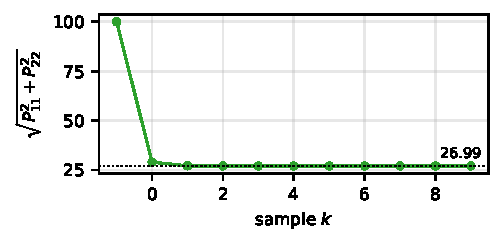
\includegraphics[width=\columnwidth]{traza_p.pdf}
\caption{Norm of the diagonal of the Kalman filter covariance on the Pico; $k=-1$ corresponds to $P_0$.}
\label{fig:traza}
\end{figure}

\subsection{Position Control of the Elbow (Additional Work)}
Fig.~\ref{fig:pid} compares a step from 0.5 to \SI{2.0}{rad} measured on the elbow with the simulation of the design. The shape of the response matches: in both cases the voltage saturates at \SI{6}{V} for about \SI{0.3}{s} and the elbow arrives without overshoot. The difference is in steady state: on the robot the controller holds \SI{\approx2}{V} to keep the position, and in simulation \SI{0}{V}.

\begin{figure}[!t]
\centering
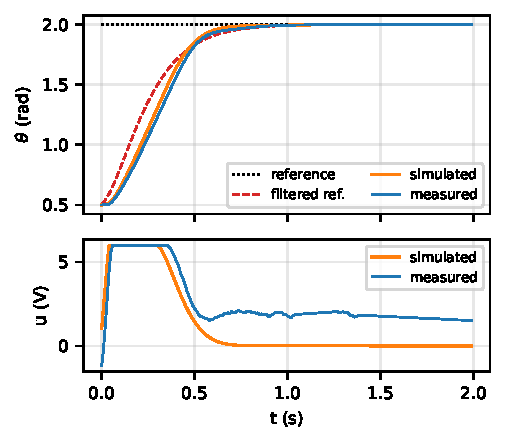
\includegraphics[width=\columnwidth]{pid_escalon.pdf}
\caption{Step from 0.5 to \SI{2.0}{rad} with $V_{max}=\SI{6}{V}$: simulated design and measurement on the elbow.}
\label{fig:pid}
\end{figure}

Fig.~\ref{fig:posreal} shows a run in which the reference was changed live from the interface, between 0.5, 1.0 and \SI{2.0}{rad}. The observers keep working in closed loop: the estimated current shows a \SIrange{1.5}{1.8}{A} peak when starting and a negative one when braking at each change, and between changes it stays at \SIrange{0.4}{0.7}{A} with a sign that depends on the position, like the voltage held by the controller.

\begin{figure}[!t]
\centering
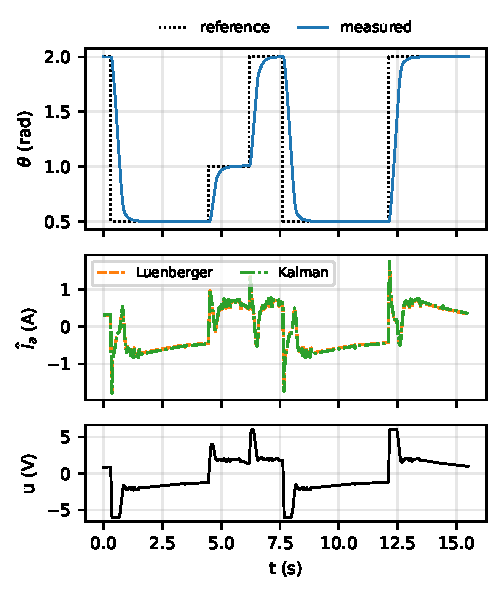
\includegraphics[width=\columnwidth]{pos_real.pdf}
\caption{Position control of the elbow with live reference changes: angle, current estimated by both observers and applied voltage.}
\label{fig:posreal}
\end{figure}

Table~\ref{tab:pos} summarizes 27 complete steps from 0.5 to \SI{1.73}{rad} measured in five runs with the shoulder held. The settling time (\SI{2}{\percent} band) was \SIrange{0.74}{0.85}{s}, about \SI{0.1}{s} longer than in simulation, and the overshoot never exceeded \SI{9.1}{mrad} (less than \SI{1}{\percent}).

\begin{table}[!t]
\centering
\caption{Position Control Performance ($V_{max}=\SI{6}{V}$)}
\label{tab:pos}
\begin{tabular}{lccc}
\toprule
 & Design & \multicolumn{2}{c}{Measured on the elbow} \\
 & (simulation) & Not saturated & Saturated \\
\midrule
Steps & -- & 18 & 9 \\
Amplitude (\si{rad}) & 0.5--2.2 & 0.50--0.72 & 1.00--1.73 \\
$t_s$ \SI{2}{\percent} (\si{s}) & 0.65--0.75 & 0.75--0.85 & 0.74--0.77 \\
Max. overshoot (\si{mrad}) & 0 & 4.7 & 9.1 \\
Mean final error (\si{mrad}) & 0 & 2.1 & 1.2 \\
Max. final error (\si{mrad}) & 0 & 4.7 & 3.9 \\
\bottomrule
\end{tabular}
\end{table}

\section{Discussion}
Tuning the model was necessary: the Lab~1 model did not meet the nominal condition because its armature resistance was about 30 times larger than expected. By fixing $K_v$ and $\beta$ from the steady-state conditions and fitting only $J$ and $L_a$, the model meets the manufacturer's specification and reproduces the measured dynamics. The remaining error is due to dry friction, which is not linear.

For the Luenberger observer, the choice of poles turned out to be decisive. With $T_s=\SI{10}{ms}$ the electrical mode of the plant is practically instantaneous, and an observer pole far from $z=0$ makes the current estimate very sensitive to model errors. The Kalman filter, on the other hand, computes its gain from $Q$ and $R$ without choosing poles by hand, and it behaved well from the first design. Its covariance converges in three samples and remains constant; for it to react to changes in the operating conditions, $Q$ or $R$ would have to vary in time, as in an adaptive filter.

With the motor braked, the estimated speed does not reach zero (Fig.~\ref{fig:pert}): neither model includes the load torque, so the observer expects the motor to turn whenever voltage is applied. Kalman suffers less from this bias because its gain on the speed ($0.77$) gives more weight to the measurement. The same effect appears in closed loop: to hold the elbow still the controller applies \SI{\approx2}{V}, with opposite sign at 0.5 and at \SI{2.0}{rad}, which indicates an external torque toward the middle of the travel, probably from the cables. The integral action compensates that torque without error, but the observers interpret it as current with the motor at rest. Adding the load torque as a third state would solve both issues.

The $z$-plane design held on the robot: the shape of the response and the overshoot match the simulation, and the settling time is only \SI{0.1}{s} longer. That difference and the final error of a few milliradians are due to dry friction, which the linear model does not include: near the reference the voltage is small and the elbow stops before arriving. In one run, the integral action kept raising the voltage against that friction with a \SI{4.5}{mrad} error until it exceeded \SI{4}{V}, and the stall protection stopped the run even though the elbow had arrived. The prefilter was essential: without it, the high $q_0$ makes the voltage swing between both saturation limits at every reference change.

A limitation of the setup also appeared in practice: when the direction was reversed with the motor at high speed, the current peak and the energy returned by the motor shut down the power supply. The open-loop experiments were therefore limited to reversals of $\pm\SI{6}{V}$ or less in the middle of the elbow travel, and the position controller was saturated at \SI{6}{V}.

\section{Conclusions}
\begin{itemize}
\item With a single speed measurement, both observers reconstruct the armature current consistently, in steady state, in transients, under load and with the motor in closed loop.
\item Under disturbances, the Kalman filter tracks the speed about four times better than the Luenberger observer (7.8 versus \SI{34.8}{rad/s} RMS) and filters the encoder quantization noise. Its covariance converges in three samples to a constant value.
\item The Luenberger design depends on the chosen poles. Modes much faster than the sampling period should be kept at $z\approx0$; the same criterion allowed reducing the position plant to second order.
\item The discrete PID designed by pole placement in $z$ met its design on the robot: over 27 steps it settled in \SIrange{0.74}{0.85}{s} with less than \SI{1}{\percent} overshoot and a mean final error of \SI{1.8}{mrad}. The prefilter and the anti-windup were necessary because of the actuator saturation.
\item The Raspberry Pi Pico runs both observers, the controller and the data acquisition in a \SI{10}{ms} loop without difficulty, which makes it a low-cost alternative to the myRIO board.
\end{itemize}

\begin{thebibliography}{9}
\bibitem{guia} M. Giraldo, ``Laboratory 4: State observers and estimators,'' Digital Control, Universidad EIA, 2026.
\bibitem{guiaeia} J. Cossio, S. Neumann and M. A. Giraldo, ``Guía práctica para la implementación de observadores de estado discretos,'' Universidad EIA.
\bibitem{pololu} Pololu Corporation, ``37D Metal Gearmotors,'' datasheet, rev. 1.2.
\bibitem{ogata} K. Ogata, \emph{Modern Control Engineering}, 5th ed. Prentice Hall, 2010.
\bibitem{welch} G. Welch and G. Bishop, ``An introduction to the Kalman filter,'' UNC Chapel Hill, 1995.
\bibitem{astrom} K. J. Åström and B. Wittenmark, \emph{Computer-Controlled Systems: Theory and Design}, 3rd ed. Prentice Hall, 1997.
\end{thebibliography}

\end{document}
